
\section{Расчёт оптимального наблюдателя}

Задан линейный объект управления
\[
\dot{\bm x}=A\bm x+\bm b u+Gw,\quad
y=C\bm x+v
\]

Матрицы системы и параметры шумов имеют вид
\[
A=\begin{pmatrix}
0&1\\
-9&-2
\end{pmatrix},
\qquad
\bm b=\begin{pmatrix}8\\4\end{pmatrix},
\qquad
W=\begin{pmatrix}7&4\\4&5\end{pmatrix},
\qquad V=4
\]

\[
C=\begin{pmatrix}1&0\end{pmatrix},
\qquad
G=I=\begin{pmatrix}1&0\\0&1\end{pmatrix}
\]

Оптимальный наблюдатель имеет вид
\[
\dot{\hat{\bm x}}=
A\hat{\bm x}+\bm b u+L(y-C\hat{\bm x})
\]

Матрица $L$ определяется из уравнения Риккати
\[
AP+PA^T+GWG^T-PC^TV^{-1}CP=0
\]

\[
L=PC^TV^{-1}
\]

Матрицу $P$ представим в симметричном виде
\[
P=\begin{pmatrix}
p_{11}&p_{12}\\
p_{12}&p_{22}
\end{pmatrix}
\]

Вычислим слагаемые уравнения Риккати
\[
\begin{aligned}
AP+PA^T
&=
\begin{pmatrix}
0&1\\-9&-2
\end{pmatrix}P+
P\begin{pmatrix}
0&-9\\1&-2
\end{pmatrix}=
\begin{pmatrix}
2p_{12}&p_{22}-9p_{11}-2p_{12}\\
p_{22}-9p_{11}-2p_{12}&-18p_{12}-4p_{22}
\end{pmatrix}
\end{aligned}
\]

Поскольку $G=I$, имеем
\[
GWG^T=W=
\begin{pmatrix}7&4\\4&5\end{pmatrix}
\]

\[
\begin{aligned}
PC^TV^{-1}CP
&=\frac14
\begin{pmatrix}
p_{11}&p_{12}\\
p_{12}&p_{22}
\end{pmatrix}
\begin{pmatrix}1\\0\end{pmatrix}
\begin{pmatrix}1&0\end{pmatrix}P=\frac14
\begin{pmatrix}
p_{11}^2&p_{11}p_{12}\\
p_{11}p_{12}&p_{12}^2
\end{pmatrix}
\end{aligned}
\]

Подставляя полученные выражения в уравнение
Риккати, получаем систему трёх нелинейных уравнений
\[
\begin{cases}
2p_{12}+7-\dfrac{p_{11}^2}{4}=0\\[3mm]
p_{22}-9p_{11}-2p_{12}+4
-\dfrac{p_{11}p_{12}}{4}=0\\[3mm]
-18p_{12}-4p_{22}+5
-\dfrac{p_{12}^2}{4}=0
\end{cases}
\]

Из первого и второго уравнений выражаем
\[
p_{12}=\frac{p_{11}^2-28}{8}
\]

\[
p_{22}=9p_{11}+2p_{12}-4+
\frac{p_{11}p_{12}}{4}
\]

Подставляя полученные выражения в третье
уравнение, получаем
\[
p_{11}^4+32p_{11}^3+776p_{11}^2
+8320p_{11}-27888=0
\]

Представим уравнение в виде
\[
(p_{11}+8)^4+392(p_{11}+8)^2-57072=0
\]

Выбирая положительный корень, получаем
\[
p_{11}=-8+2\sqrt{4\sqrt{373}-49}
\approx2{,}630679
\]

Остальные элементы матрицы
\[
p_{12}=\frac{p_{11}^2-28}{8}
\approx-2{,}634941
\]

\[
p_{22}=9p_{11}+2p_{12}-4+
\frac{p_{11}p_{12}}{4}
\approx12{,}673304
\]

Таким образом
\[
P\approx
\begin{pmatrix}
2{,}630679&-2{,}634941\\
-2{,}634941&12{,}673304
\end{pmatrix}
\]

Проверим положительную определённость матрицы $P$
\[
p_{11}\approx2{,}630679>0
\]

\[
\det P\approx26{,}396472>0
\]

Следовательно
\[
P\succ0
\]

Коэффициенты оптимального наблюдателя
\[
L=PC^TV^{-1}
\]

\[
\begin{aligned}
L
&=
\begin{pmatrix}
2{,}630679&-2{,}634941\\
-2{,}634941&12{,}673304
\end{pmatrix}
\begin{pmatrix}1\\0\end{pmatrix}
\frac14\approx
\begin{pmatrix}
0{,}657670\\
-0{,}658735
\end{pmatrix}
\end{aligned}
\]

Полученный оптимальный наблюдатель имеет вид
\[
\dot{\hat{\bm x}}=
\begin{pmatrix}0&1\\-9&-2\end{pmatrix}
\hat{\bm x}
+
\begin{pmatrix}8\\4\end{pmatrix}u
+
\begin{pmatrix}
0{,}657670\\-0{,}658735
\end{pmatrix}
(y-C\hat{\bm x})
\]

\subsection{Моделирование оптимального наблюдателя}

Проведем моделирование оптимального наблюдателя при начальных условиях
\[
x(0)=\begin{pmatrix}1\\0\end{pmatrix},
\qquad
\hat{x}(0)=\begin{pmatrix}0\\0\end{pmatrix}
\]

В качестве управляющего воздействия возьмём сигнал
\[
u(t)=\sin t
\]

Для оценки математического ожидания квадратичной ошибки применён метод Монте-Карло с $10^7$ реализаций случайных возмущений.

На рисунке~\ref{fig:task5_errors} представлены графики ошибок оценивания состояний $e_{H1}(t)$ и $e_{H2}(t)$.

\begin{figure}[H]
    \centering
    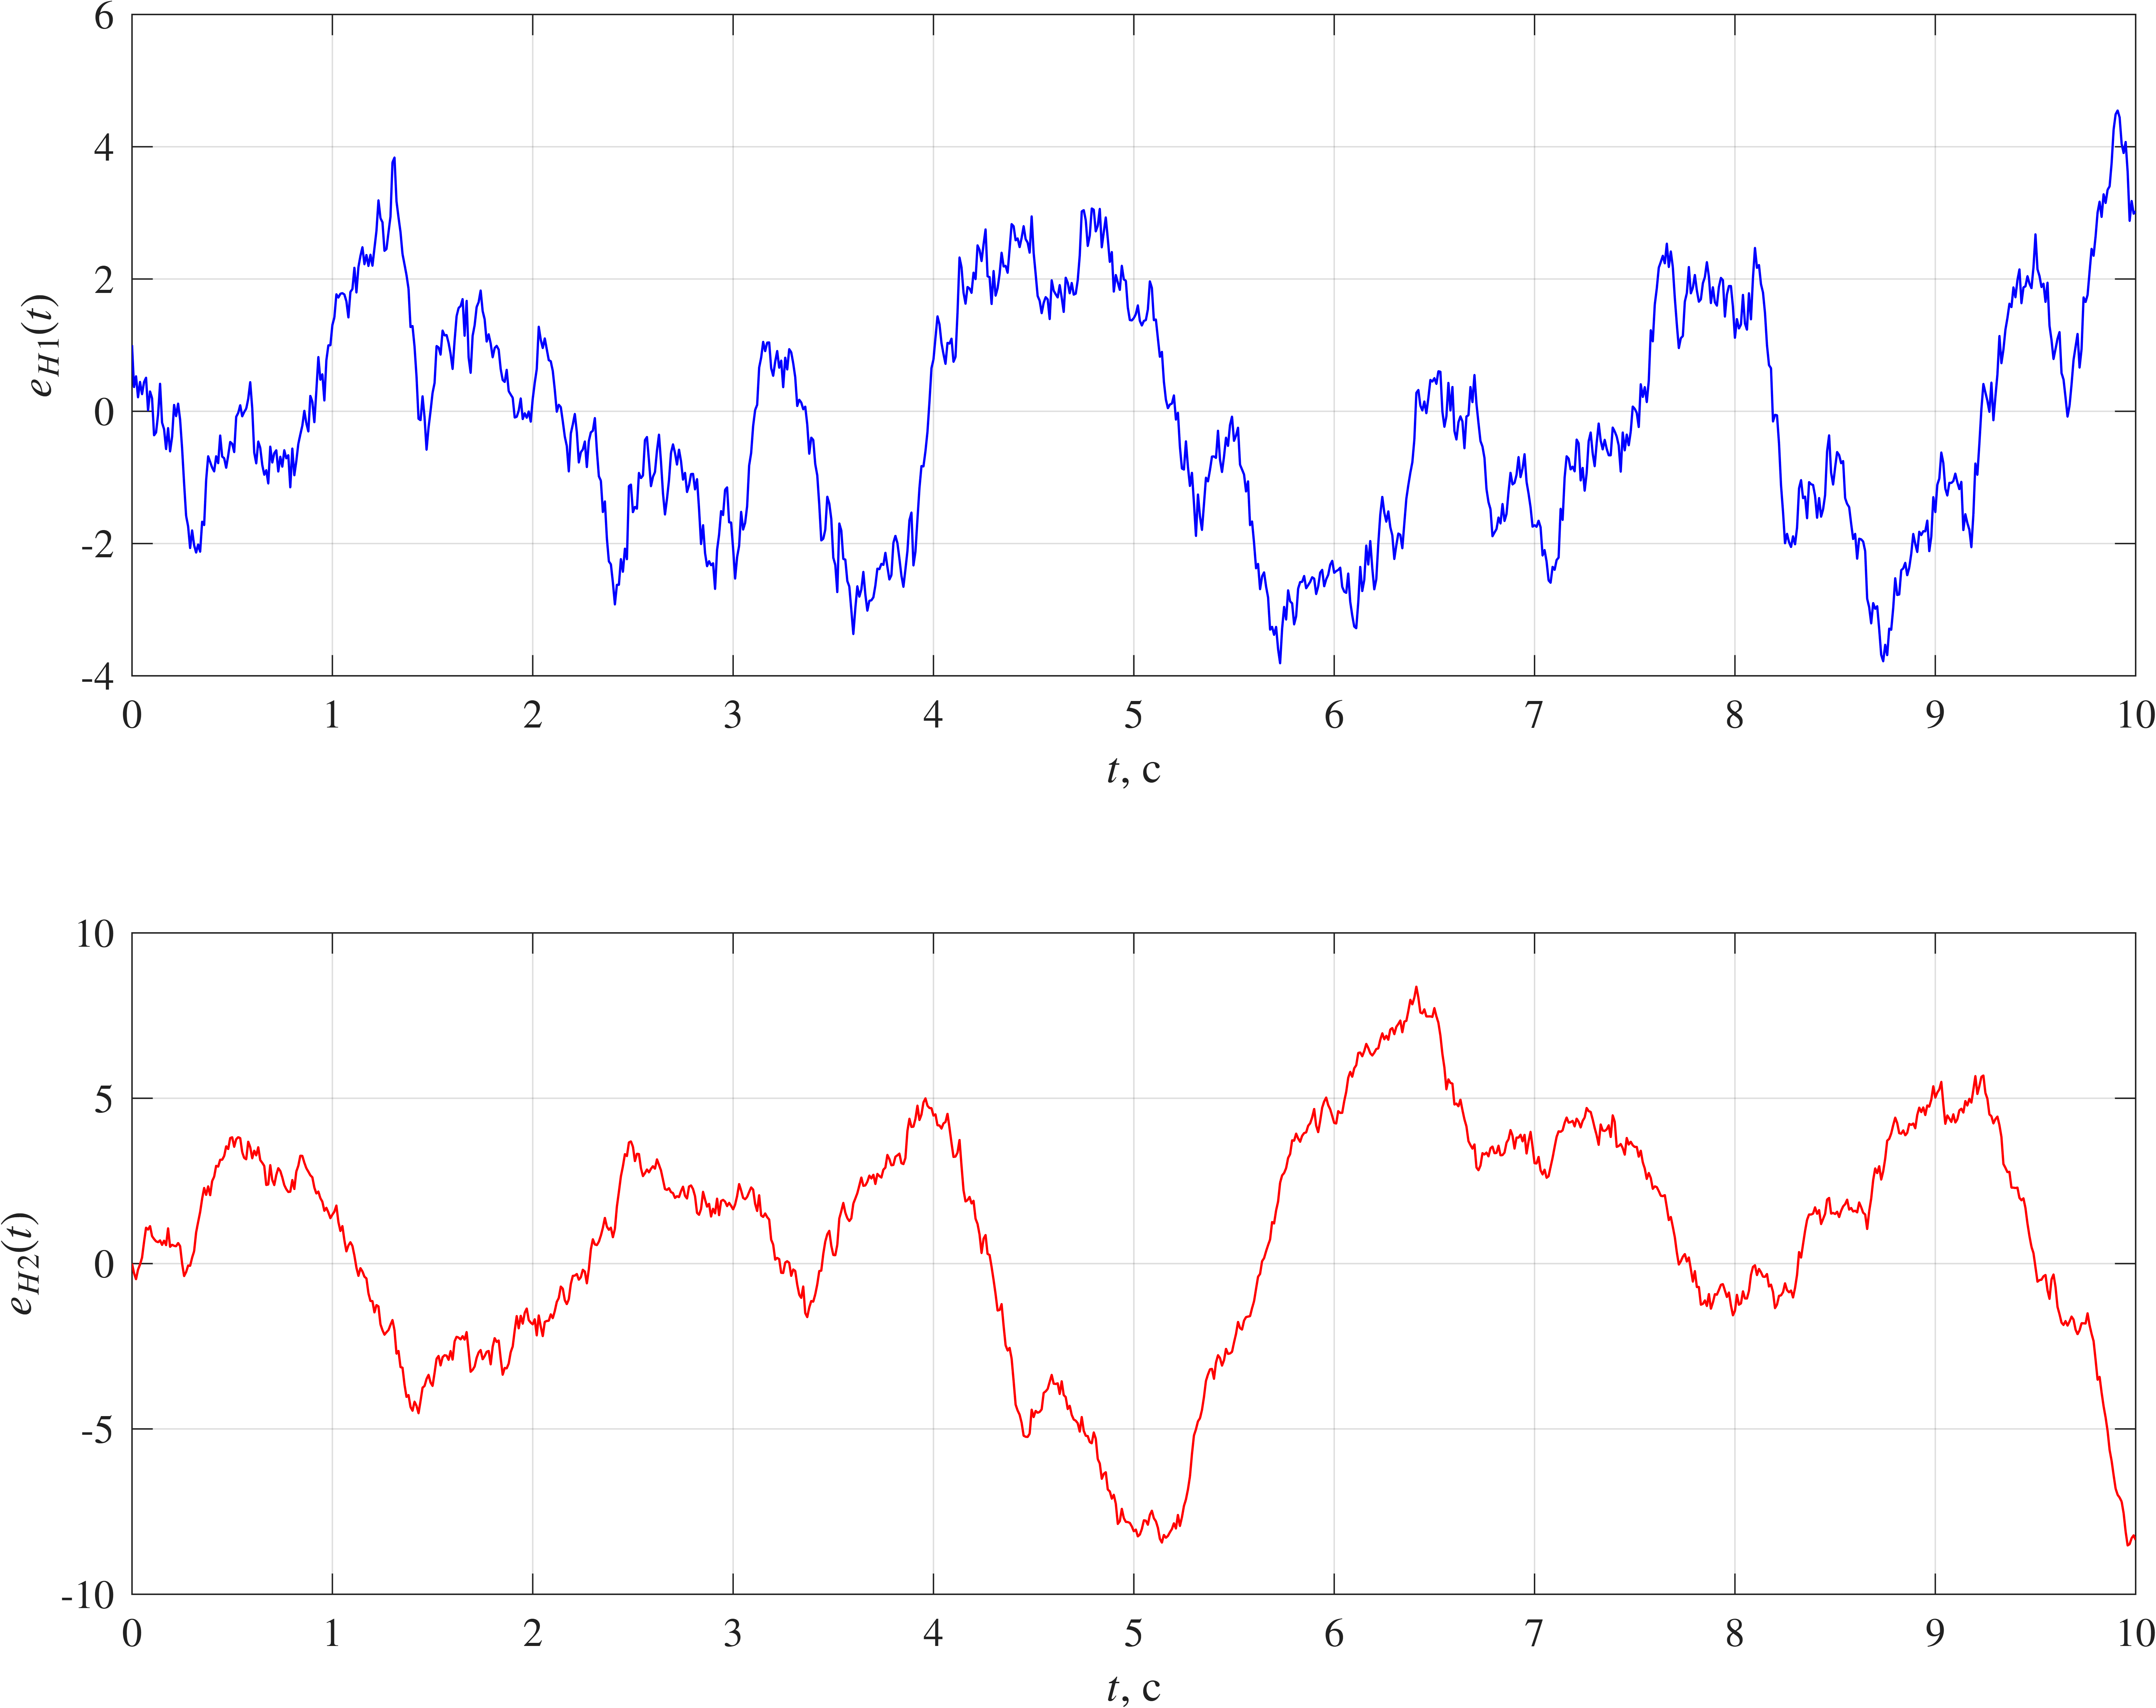
\includegraphics[width=0.9\textwidth]{images/task5_errors.png}
    \caption{Ошибки оценивания состояний оптимальным наблюдателем}
    \label{fig:task5_errors}
\end{figure}

Ошибки оценивания изменяются случайным образом и колеблются относительно нуля. Отсутствие их сходимости к нулю объясняется непрерывным воздействием шумов объекта и измерения.

Критерий качества наблюдателя определяется математическим ожиданием суммы квадратов ошибок:
\[
J(t)=M\left\{e_{H1}^2(t)+e_{H2}^2(t)\right\}
\]

Результат его вычисления представлен на рисунке~\ref{fig:task5_J}.

\begin{figure}[H]
    \centering
    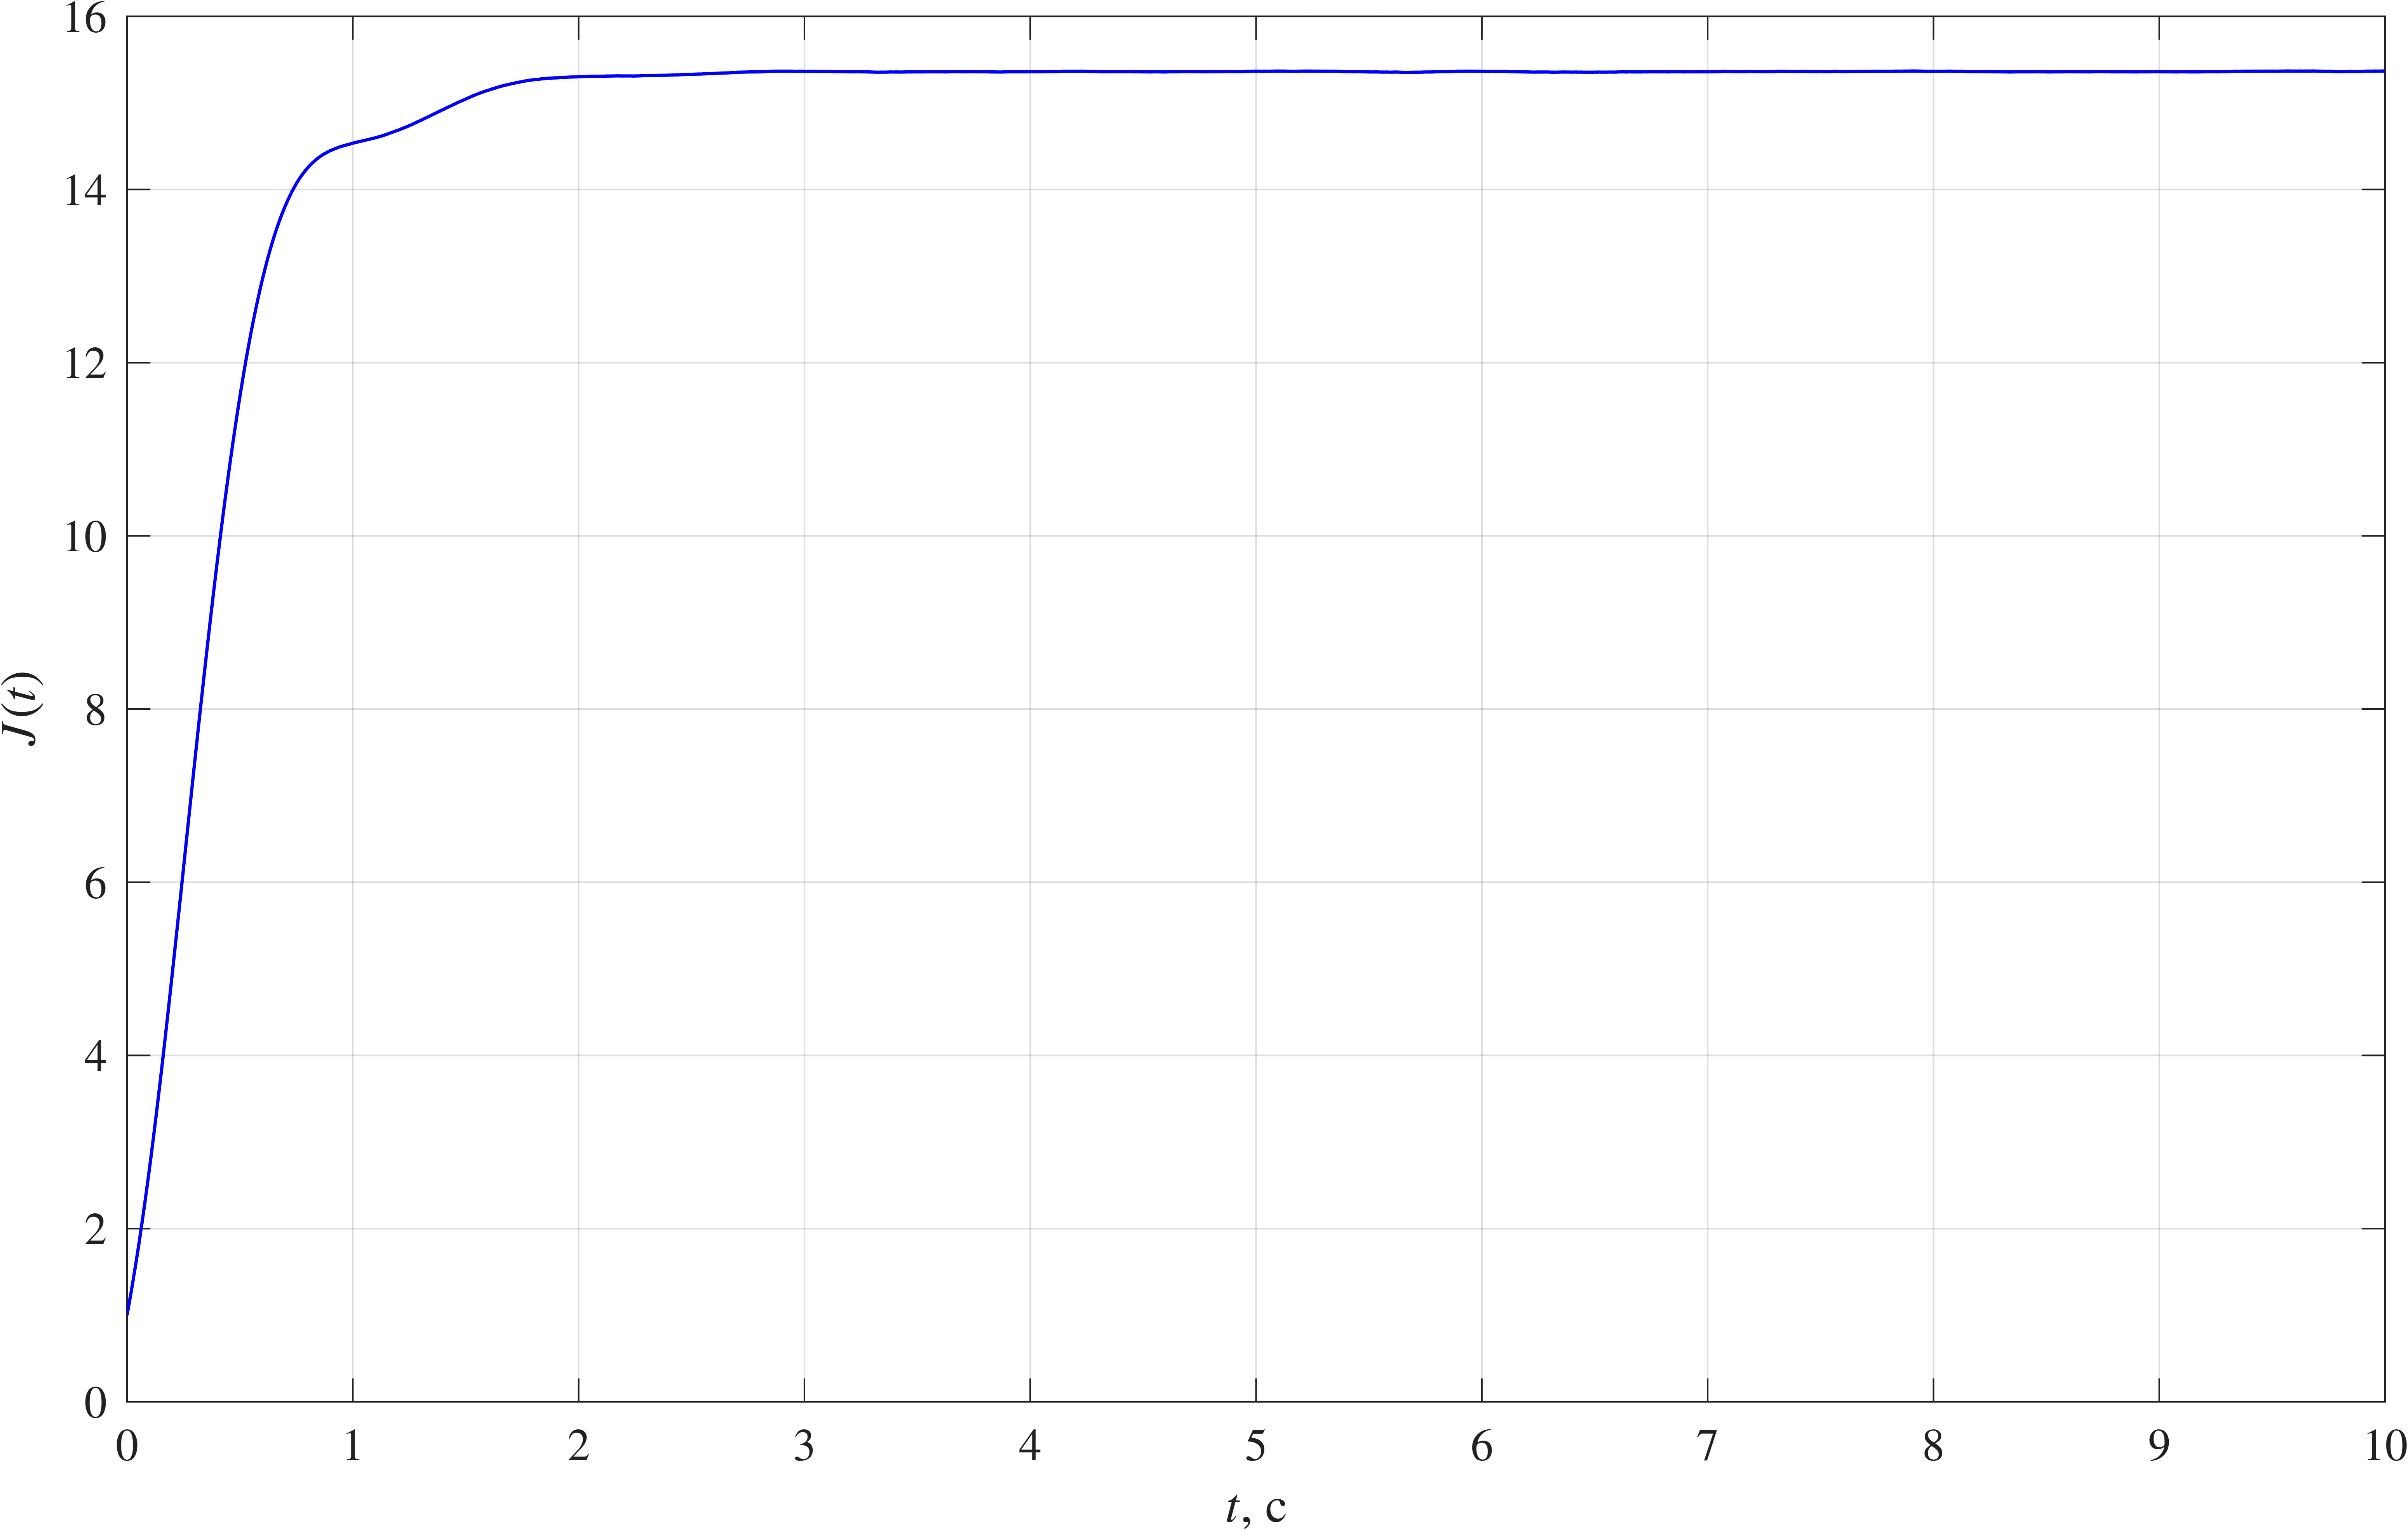
\includegraphics[width=0.9\textwidth]{images/task5_J.png}
    \caption{Математическое ожидание квадратичной ошибки наблюдения}
    \label{fig:task5_J}
\end{figure}

В начальный момент времени значение критерия равно $J(0)=1$, что соответствует заданным начальным условиям. В дальнейшем критерий возрастает и приблизительно к $t=2$~с достигает установившегося значения.
